\subsection{Impendantie driehoek}
Voor de impendantie is ook een driehoek te maken. Dit is de driehoek voor een spoel.

\begin{center}

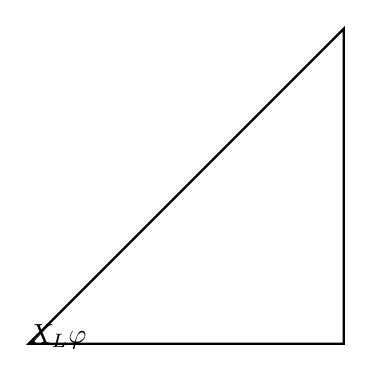
\begin{tikzpicture}[thick]
\coordinate (O) at (0,0);
\coordinate (A) at (4,0);
\coordinate (B) at (4,4);
\draw (O)--(A)--(B)--cycle;

\tkzLabelSegment[below=2pt](O,A){\textit{R}}
\tkzLabelSegment[left=2pt](O,B){\textit{Z}}
\tkzLabelSegment[above right=2pt](A,B){\textit{$X_L$}}

\tkzMarkAngle[fill= teal,size=0.8cm,%
opacity=.4](A,O,B)
\tkzLabelAngle[pos = 0.6](A,O,B){$\varphi $}

\end{tikzpicture}
\end{center}

Hier geldt:\\
R= weerstand\\
Z= impendantie\\
$X_L$= inductieve reactantie\\

De verschillen de waardes kunnen bepaald worden op de zelfde manier als bij de vermogensdriehoek.

\vspace{5mm}

Voor de Condensator geld het zelfde alleen is $X_L$ vervangen door $X_C$ en is de impendantie negatief.

\begin{center}

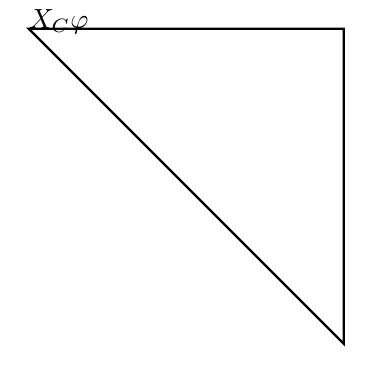
\begin{tikzpicture}[thick]
\coordinate (O) at (0,0);
\coordinate (A) at (4,0);
\coordinate (B) at (4,-4);
\draw (O)--(A)--(B)--cycle;

\tkzLabelSegment[above=2pt](O,A){\textit{R}}
\tkzLabelSegment[left=2pt](O,B){\textit{Z}}
\tkzLabelSegment[above right=2pt](A,B){\textit{$X_C$}}

\tkzMarkAngle[fill= teal,size=0.8cm,%
opacity=.4](B,O,A)
\tkzLabelAngle[pos = -0.6](A,O,B){$\varphi $}

\end{tikzpicture}
\end{center}